\chapter{Formulation relativiste}


{\small \it Note : la première partie se trouve sur une feuille distribuée par le professeur.}
\section{Rappels d'analyse tensorielle}
\section{Formulation relativiste de l'électrodynamique}
\subsection{Postulats fondamentaux}

\begin{postulat}
	Les lois de la physique, lorsqu'elles sont formulées de manière adéquate, gardent la m\^eme forme dans un référentiel $\mathcal{R}$ et dans un référentiel $\mathcal{R}'$ en translation rectiligne uniforme par rapport à $\mathcal{R}$. Il y a invariance de la forme des équations.\\
	Contribution d'Einstein : la vitesse de propagation d'un signal électromagnétique dans le vide est universelle et indépendante du référentiel.
\end{postulat}

\begin{cons}
	Ce sont les équations de Maxwell qui sont invariantes, et cela a donc amené à abandonner la mécanique classique (Newtonienne) pour la reformuler afin qu'elle soit aussi invariante sous une transformation de Lorentz.
\end{cons}

\begin{postulat}
	Invariance de la charge : en accord avec les expériences, on postule que la charge q d'une particule ne dépend pas du référentiel galiléen considéré.
\end{postulat}

\begin{cons}
	L'invariance formelle des lois de la physique est automatiquement satisfaite si on les écrit sous forme temporelle (condition suffisante), sachant que les transformations à considérer sont les transformations du groupe de Lorentz, qui recouvre les translations spatiales et temporelles, les rotations, les renversements d'axe, et les boosts de Lorentz.
$$
	x'^{\mu}=\mathcal{L}^{\mu}_{\nu}x^{\mu} \text{ avec }\mathcal{L}^{\mu}_{\nu}=\begin{mat}
	\gamma & -\beta\gamma & \hspace*{0.2cm}0\hspace*{0.2cm} \\
	-\beta\gamma & \gamma & \hspace*{0.2cm}0\hspace*{0.2cm} \\
	0 & 0 & \hspace*{0.2cm}1\hspace*{0.2cm}
	\end{mat}
$$
\end{cons}


\subsection{Quadrivecteur courant}
{\txt
On cherche à construire un quadrivecteur à partir de $\rho$ et $\vec{j}$. Ainsi, on considère une charge $q$ dans un référentiel $\mathcal{R}$, que l'on modélise comme une distribution de charge $\rho$ dans un volume $\dif V=\frac{q}{\rho}$. Dans $\mathcal{R}'$ en translation rectiligne uniforme par rapport à $\mathcal{R}$, cette charge $q$ occupe $\dif V'$ et correspond à $\rho'$. D'après le postulat d'invariance de la charge, on a : $\rho \,\dif V=q=\rho'\, \dif V'$. Dans $\mathcal{R}$, la charge est en mouvement et est donc associée à un vecteur densité de courant :}
$$
	\vec{j}=\begin{cases}
		\rho\vec{v}&\text{si }\vec{r}\in \dif V\\
		\vec{0}&\text{sinon}
	\end{cases}
$$

{\txt
Pendant un intervalle de temps $\dif t$ dans $\mathcal{R}$, la charge se déplace de $\dif x^\mu=(\dif t,\dif\vec{r})$. $\dif x^\mu$ étant un quadrivecteur, il en est de m\^eme pour $\rho \,\dif V\dif x^\mu$. On considère alors $\rho\frac{c\,\dif t\,\dif V}{c}\frac{\dif x^\mu}{\dif t}$}.

\begin{postulat}
	$c\,\dif t\,\dif V$ est un invariant.
\end{postulat}

\begin{proof}
	$c\,\dif t\,\dif V$ étant l'élément d'intégration dans l'espace de Minkovski, on considère la matrice jacobienne.
\begin{rappel}
	Soit $\varphi:(x,y,z)\longrightarrow \vec{\varphi}(x,y,z)=\begin{mat}
		u(x,y,z)\\
		v\\
		w
	\end{mat}$
	
	$$
		\text{Jac}_\varphi=\frac{D(u,v,w)}{D(x,y,z)}=\begin{mat}
			\partial_xu & \partial_yu & \partial_zu\\
			\partial_xv & \partial_yv & \partial_zv\\
			\partial_xw & \partial_yw & \partial_zw
		\end{mat}\\
	$$
	$$
		J_\varphi=\det(\text{Jac}_\varphi)
	$$
	$$
		\text{alors }\bigintssss_{\varphi(x)}f(u_1,...u_n)\,\dif u_1...\,\dif u_n=\bigintssss_Xf\circ\varphi(x_1,...x_n)|J_\varphi|\,\dif x_1...\,\dif x_n
	$$
\end{rappel}
Pour un boost de Lorentz, on a :
$$
	\begin{mat}
		ct' \\ x' \\ y' \\ z'
	\end{mat}
	=
	\begin{mat}
		\gamma & -\beta\gamma & 0 & 0\\
		-\beta\gamma & \gamma & 0 & 0\\
		0 & 0 & 1 & 0\\
		0 & 0 & 0 & 1
	\end{mat}
	\begin{mat}
		ct \\ x \\ y \\ z
	\end{mat}
	\text{ et par conséquent }J_{boost}=1
$$
$$
	\begin{array}{r@{\;}l}
		\text{d'où\hspace*{0.5cm}} c\,\dif t\,\dif x\,\dif y\,\dif z&=c\,\dif t'\,\dif x'\,\dif y'\,\dif z'\\
		c\,\dif t\,\dif V&=c\,\dif t'\,\dif V'
	\end{array}
$$
\end{proof}

\begin{remark}
{\txt Attention aux démonstrations avec $\dif t'=\gamma \dif t$ et $\dif x'=\frac{1}{\gamma}\dif x$}
\end{remark}

\begin{corol}
	{\txt $c\,\dif t\,\dif x\,\dif y\,\dif z$ est invariant et donc $\rho\frac{\dif x^\mu}{\dif t}$ est un quadrivecteur.}\\
	On pose $J^\mu=\rho\frac{\dif x^\mu}{\dif t}$ le quadrivecteur courant (composantes contravariantes).\\
	$J^\mu=(\rho c,\vec{j})=(\rho c,\rho \vec{v})=\rho_0(\gamma c,\gamma\vec{v})$ où $\rho_0$ est la densité de charges dans le référentiel propre de la particule.
\end{corol}

\subsection{Formulation covariante de l'électromagnétisme}
\subsubsection{Retour sur un opérateur}

On a vu que $\nabla$ est un quadrivecteur dont les composantes covariantes sont $\partial_a=\frac{\partial}{\partial{x^a}}$ soit :
$$ 
	\nabla=\left(\frac{1}{c}\frac{\partial}{\partial t},\frac{\partial}{\partial x},\frac{\partial}{\partial y},\frac{\partial}{\partial z}\right)
$$
et ses composantes contravariantes s'écrivent : $\left(\frac{1}{c}\frac{\partial}{\partial t},-\frac{\partial}{\partial x},-\frac{\partial}{\partial y},-\frac{\partial}{\partial z}\right)$\\
$\partial^a\partial_a$ est un tenseur d'ordre 0 obtenu par contraction de deux tenseurs de rang 1 et est donc invariant.
$$
	\begin{array}{r@{\;}l}
			\partial^a\partial_a&=\partial^0\partial_0+\partial^1\partial_1+\partial^2\partial_2+\partial^3\partial_3\\
		&=\frac{1}{c^2}\frac{\partial^2}{\partial t^2}-\frac{\partial^2}{\partial x^2}-\frac{\partial^2}{\partial y^2}-\frac{\partial^2}{\partial z^2} = -\square
	\end{array}	
$$

\subsubsection{Quadrivecteur potentiel}
En jauge de Lorenz ($\nab\cdot\vec{A}+\frac{1}{c^2}\partial_t\phi=0$), les équations satisfaites par les potentiels sont :
$$
	\left\{ \begin{array}{l}
		\nab^2\phi - \frac{1}{c^2}\partial_t^2\phi=-\frac{\rho}{\epsilon_0}\\
		\nab^2\vec{A}-\frac{1}{c^2}\partial_t^2\vec{A}=-\mu_0\vec{j}\\
		\square\,\frac{\phi}{c}=-\frac{\rho}{c\epsilon_0}=-\mu_0\rho c\\
		\square\,\vec{A}=-\mu_0\vec{j}
	\end{array} \right.
$$
{\txt On est amené à considérer $(\frac{\phi}{c},\vec{A})$ comme les composantes contravariantes d'un quadrivecteur, le quadri-potentiel.}
$$
	\square\,\phi^\mu=-\mu_0J^\mu
	\text{ avec } \phi^\mu=(\frac{\phi}{c},\vec{A})
$$
En ce qui concerne la jauge de Lorenz,
$$
	\begin{array}{r@{\;}l}
		0&=\nab\cdot\vec{A}+\frac{1}{c^2}\partial_t\phi=\partial_\mu\phi^\mu\\
		&=\partial_0\phi^0+\partial_1\phi^1+\partial_2\phi^2+\partial_3\phi^3\\
		&=\frac{1}{c}\partial_t\left(\frac{\phi}{c}\right)+\underbrace{\partial_xA_x+\partial_yA_y+\partial_zA_z}_{\nab\cdot\vec{A}}
	\end{array}
$$
La jauge est covariante.

\begin{conc}
	On a été capable de reformuler l'électromagnétique sous forme covariante :
	$$
		\left\{ \begin{array}{r@{\;}l}
			\partial_\mu\phi^\mu&=0\text{\hspace{1cm}(jauge)}\\
			\square\,\phi^\mu&=-\mu_0J^\mu
		\end{array} \right.
	$$
\end{conc}

\subsubsection{Équation de Maxwell-Lorentz}
	Les quadrivecteurs ont quatre composantes, alors que $\vec{E}$ et $\vec{B}$ n'en ont chacun que trois. Il est nécessaire de considérer un tenseur d'ordre supérieur ou égal à 2. On part de l'expression de $\vec{E}$ et $\vec{B}$ avec les potentiels :

$$
	\vec{B}=\nab\times\vec{A}\text{\hspace{1cm}et\hspace{1cm}}\vec{E}=-\nab\phi-\partial_t\vec{A}
$$
$$
	\begin{array}{r@{\;}l@{\;}l}
		B_x & = \partial_y A_z - \partial_z A_y = \partial_2 \phi^3 - \partial_3 \phi^2 & = - (\partial_3 \phi^2 - \partial_2 \phi^3) \\
		B_y & = \partial_x A_z - \partial_z A_x = \partial_1 \phi^3 - \partial_3 \phi^1 & = - (\partial_3 \phi^1 - \partial_1 \phi^3) \\
		B_z & = \partial_y A_x - \partial_x A_y = \partial_2 \phi^1 - \partial_1 \phi^2 & = - (\partial_1 \phi^2 - \partial_2 \phi^1) \\	
		E_x & = - \partial_x \phi - \partial_t A_x = \partial_1 \phi^0 - \partial_0 \phi^1 & = - (\partial_0 \phi^1 - \partial_1 \phi^0) \\
		E_y & = - \partial_y \phi - \partial_t A_y = \partial_2 \phi^0 - \partial_0 \phi^2 & = - (\partial_0 \phi^2 - \partial_2 \phi^0) \\
		E_z & = - \partial_z \phi - \partial_t A_z = \partial_3 \phi^0 - \partial_0 \phi^3 & = - (\partial_0 \phi^3 - \partial_3 \phi^0)
	\end{array}
$$

{\txt $\frac{E_x}{c}$,$\frac{E_y}{c}$,$\frac{E_z}{c}$,$B_x$,$B_y$,$B_z$ apparaissent donc comme les composantes d'un tenseur d'ordre deux asymétrique :}
$$
	\begin{array}{r@{\;}l}
		F^{\mu\nu}&=\partial^\mu\phi^\nu-\partial^\nu\phi^\mu\\
		F^{\mu\nu}&=\begin{mat}[1.7]
			0 & -\frac{E_x}{c} & -\frac{E_y}{c} & -\frac{E_z}{c}\\
			\frac{E_x}{c} & 0 & -B_z & B_y \\
			\frac{E_y}{c} & B_z & 0 & -B_x \\
			\frac{E_z}{c} & -B_y & B_x & 0 
		\end{mat}
	\end{array}
$$
Les coordonnées covariantes de ce tenseur sont :
$$
	F_{\mu\nu}=g_{\mu\alpha}g_{\nu\beta}F^{\alpha\beta}=\begin{mat}[1.7]
		0 & \frac{E_x}{c} & \frac{E_y}{c} & \frac{E_z}{c}\\
		-\frac{E_x}{c} & 0 & -B_z & B_y \\
		-\frac{E_y}{c} & B_z & 0 & -B_x \\
		-\frac{E_z}{c} & -B_y & B_x & 0
	\end{mat}
$$
On exprime alors les équations de Maxwell sous forme covariante :

\begin{minipage}{0.35\linewidth}
$$\nab\cdot\vec{E}=\frac{\rho}{\epsilon_0} \text{\hspace{1.5cm}}$$
\end{minipage}
\begin{minipage}{0.55\linewidth}
$
	\begin{array}{r@{\;}l}
		\partial_\mu F^{\mu 0}&=\partial_0F^{00}+\partial_1F^{10}+\partial_2F^{20}+\partial_3F^{30}\\
		&=0+\partial_x\left(\frac{E_x}{c}\right)+\partial_y\left(\frac{E_y}{c}\right)+\partial_z\left(\frac{E_z}{c}\right)\\
		&=\frac{1}{c}\nab\cdot\vec{E}=\frac{\rho}{c\epsilon_0}=\mu_0J^0
	\end{array}
$
\end{minipage}
\vspace{0.5cm}

\begin{minipage}{0.35\linewidth}
$$\nab\times\vec{B}=\mu_0\vec{j}+\mu_0\epsilon_0\partial_t\vec{E} \text{\hspace{1cm}}$$
\end{minipage}
\begin{minipage}{0.55\linewidth}
$
	\begin{array}{r@{\;}l}
		\partial_\mu F^{\mu 1}&=\partial_0F^{01}+\partial_1F^{11}+\partial_2F^{21}+\partial_3F^{31}\\
		&=\partial_x\left(-\frac{E_x}{c}\right)+0+\partial_yB_z+\partial_z\left(-B_y\right)\\
		&=\left.\nab\times\vec{B}\right|_x-\frac{1}{c^2}\partial_t\left.\vec{E}\right|_x=\mu_0J_x
	\end{array}
$
\end{minipage}
\vspace{0.5cm}

\noindent De la m\^eme manière, $\partial_\mu F^{\mu 2}$ et $\partial_\mu F^{\mu 3}$ donnent les composantes $x$ et $y$ de l'équation de Maxwell-Ampère.
Pour les équations de Maxwell avec sources, on a donc :
$$
	\boxed{\partial_\mu F^{\mu\nu}=\mu_0J^\nu}
$$
sous forme covariante. Intéressons-nous aux équations de Maxwell homogènes :
$$
	\begin{array}{r@{\;}l}
		\partial_1F_{23}+\partial_2F_{31}+\partial_3F_{12}&=\partial_x(-B_x)+\partial_y(-B_y)+\partial_z(-B_z)\\
			&= -\nab\cdot\vec{B}\\
			&= 0 \\[10pt]
		\partial_0F_{32}+\partial_3F_{20}+\partial_2F_{03}&=\frac{\partial}{c\partial t}B_x+\partial_z\left(-\frac{E_y}{c}\right)+\partial_y\left(\frac{E_z}{c}\right)\\
			&=\left.\frac{\nab\cdot\vec{E}}{c}\right|_x+\frac{1}{c}\left.\frac{\partial \vec{B}}{\partial t}\right|_x
	\end{array}
$$
M\^eme chose pour $y$ et $z$. Ces équations s'écrivent alors :
$$
	\boxed{\partial_\alpha F_{\beta\gamma} + \partial_\beta F_{\gamma\alpha} + \partial_\gamma F_{\alpha\beta} = 0}
$$

\subsubsection*{Équation de Lorentz}

$$
	m\frac{\dif}{\dif t}\frac{\vec{v}}{\sqrt{1-\frac{v^2}{c^2}}}=m\frac{\dif }{\dif t}(\gamma\vec{v})=\frac{\dif }{\dif t}(\gamma m \vec{v})=q(\vec{E}+\vec{v}\times\vec{B})
$$
et
$$
	\frac{\dif}{\dif t}(\gamma m c^2)=\bigintssss\vec{j}\cdot\vec{E}=q\vec{v}\cdot\vec{E}
$$
En utilisant le fait que
$$
	\frac{\dif}{\dif t}=\frac{\dif\tau}{\dif t}\frac{\dif}{\dif\tau}=\frac{1}{\gamma}\frac{\dif}{\dif\tau}\\
$$
on obtient
$$
	\frac{\dif}{\dif\tau}\gamma\vec{v}=q\left(\gamma c\frac{\vec{E}}{c}+\gamma\vec{v}\times\vec{B}\right)
$$
et
$$
	\frac{\dif}{\dif\tau}(\gamma mc)=q\gamma\vec{v}\cdot\frac{\vec{E}}{c}
$$
Soit
$$
	\boxed{\frac{\dif P^\mu}{\dif\tau}=qF^{\mu\nu}u_\nu}
$$
{\renewcommand*{\arraystretch}{1.2}
$$
	\begin{array}{lr@{\;}ll}
		\text{o\`u }&P^\mu&=(\gamma mc,\gamma m\vec{v})=mu^\mu&\text{ composante contravariante de la quadri-impulsion}\\
		&u^\mu&=(\gamma c,\gamma\vec{v})&\text{ composante contravariante de la quadri-vitesse}\\
		&u_\mu&=(\gamma c,-\gamma\vec{v})&\text{ composante covariante de la quadri-vitesse}
	\end{array}
$$}

\begin{proof}
$$
	\begin{array}{r@{\;}l}
		F^{0\nu}u_\nu&=F^{00}U_0+F^{01}U_1+F^{02}U_2+F^{03}U_3\\
			&=0+\left(-\frac{E_x}{c}\right)(-\gamma v_x)+\left(-\frac{E_y}{c}\right)(-\gamma v_y)+\left(-\frac{E_z}{c}\right)(-\gamma v_z)\\
			&=\gamma\vec{v}\frac{\vec{E}}{c}\\[10pt]
		F^{\nu}&=...
	\end{array}
$$
\end{proof}

\begin{conc}
On a formulé les équations de Maxwell ainsi que la force de Lorentz sous forme covariante.
\end{conc}

\subsection{Résumé}

Après avois introduit
\begin{itemize}
	\item le quadri-nabla de composantes covariantes $\partial_\mu \equiv \left(\frac{\partial}{c\partial t}, \frac{\partial}{\partial x},\frac{\partial}{\partial y},\frac{\partial}{\partial z}\right)$
	\item l'opérateur d'Alembertien $\square=\nab^2-\frac{1}{c^2}\frac{\partial^2}{\partial t^2}$
	\item le quadrivecteur courant de composantes contravariantes $J^\mu=(\rho c,\vec{j})$
	\item le quadrivecteur potentiel de composantes contravariantes $\phi^\mu=\left(\frac{\phi}{c},\vec{A}\right)$
	\item le tenseur électromagnétique de composantes contravariantes $$F^{\mu\nu}=\begin{mat}[1.7]
			0 & -\frac{E_x}{c} & -\frac{E_y}{c} & -\frac{E_z}{c}\\
			\frac{E_x}{c} & 0 & -B_z & B_y \\
			\frac{E_y}{c} & B_z & 0 & -B_x \\
			\frac{E_z}{c} & -B_y & B_x & 0 
		\end{mat}$$
\end{itemize}
les équations de Maxwell prennent la forme covariante suivante :
$$
	\boxed{\square\phi^\mu+\partial^\mu(\partial_\nu\phi^\nu)=-\mu_0J^\mu}
$$
{\renewcommand*{\arraystretch}{1.2}$$
	\begin{array}{r@{\;}l}
		\iff& \left\{ \begin{array}{l}
			\square\phi^\mu=-\mu_0J^\mu\\
			\partial_\nu\phi^\nu=0\text{\hspace{0.5cm}(jauge de Lorenz)}
		\end{array}\right.\\[15pt]
		\iff& \left\{ \begin{array}{l}
			F^{\mu\nu}=\partial^\mu\phi^\nu-\partial^\nu\phi^\mu\\
			\partial_\mu F^{\mu\nu}=\mu_0J^\nu\\
			\partial_\alpha F_{\beta\gamma} + \partial_\beta F_{\gamma\alpha} + \partial_\gamma F_{\alpha\beta}=0
		\end{array}\right.
	\end{array}
$$}

En ce qui concerne l'équation de Lorentz associée à l'équation de conservation de l'énergie, elle s'écrit sous la forme covariante suivante :
$$
	\boxed{\frac{dP^\mu}{d\tau}=qF^{\mu\nu}u_\nu}
$$
{\renewcommand*{\arraystretch}{1.2}
$$
	\begin{array}{lr@{\;}l}
		\text{o\`u }&P^\mu&=(\gamma mc,\gamma m\vec{v})=mu^\mu\\
		&u^\mu&=(\gamma c,\gamma\vec{v})\\
		&u_\mu&=(\gamma c,-\gamma\vec{v})
	\end{array}
$$}

\begin{remark}
	La conservation de la charge s'écrit de façon covariante $\partial_\mu J^\mu=0$, équation bien satisfaite car $F^{\mu\nu}$ est antisymétrique.
\end{remark}

\section{Applications}
\subsection[\texorpdfstring{Formules de transformation des champs $\vec{E}$ et $\vec{B}$}{Formules de transformation des champs E et B}]{Formules de transformation des champs $\boldsymbol{\vec{E}}$ et $\boldsymbol{\vec{B}}$}
On sait comment se transforme $F^{\mu\nu}$
$$
	F'^{\mu\nu}=\frac{\partial x'^\mu}{\partial x^\alpha}\frac{\partial x'^\nu}{\partial x^\beta}F^{\alpha\beta}
$$
et on considère le boost de Lorentz correspondant à
{\renewcommand*{\arraystretch}{1.2}$$
	\left\{ \begin{array}{r@{\;}l}
		ct'&=\gamma ct-\beta\gamma x\\
		x'&=-\beta\gamma ct+\gamma x\\
		y'&=y\\
		z'&=z
	\end{array} \right.
$$}
{\renewcommand*{\arraystretch}{2}$$
	\begin{array}{r@{\;}l}
		F'^{01}=&-\frac{E'_x}{c}\\
			=&\frac{\partial x'^0}{\partial x^\alpha}\frac{\partial x'^1}{\partial x^\beta}F^{\alpha\beta}
			=\frac{\partial ct'}{\partial x^\alpha}\frac{\partial x'}{\partial x^\beta}F^{\alpha\beta}\\
			=&\frac{\partial ct'}{\partial ct}\frac{\partial x'}{\partial ct}\underbrace{F^{00}}_{=0}
				+\frac{\partial ct'}{\partial ct}\frac{\partial x'}{\partial x}F^{01}
				+\frac{\partial ct'}{\partial ct}\underbrace{\frac{\partial x'}{\partial y}}_{=0}F^{02}
				+\frac{\partial ct'}{\partial ct}\underbrace{\frac{\partial x'}{\partial z}}_{=0}F^{03}\\
			&+\frac{\partial ct'}{\partial x}\frac{\partial x'}{\partial ct}F^{10}
				+\frac{\partial ct'}{\partial x}\frac{\partial x'}{\partial x}\underbrace{F^{11}}_{=0}
				+\frac{\partial ct'}{\partial x}\underbrace{\frac{\partial x'}{\partial y}}_{=0}F^{12}
				+\frac{\partial ct'}{\partial x}\underbrace{\frac{\partial x'}{\partial z}}_{=0}F^{13}\\
			&+\left(\text{4 termes en }\frac{\partial ct'}{\partial y}\right)
				+\left(\text{4 termes en }\frac{\partial ct'}{\partial z}\right)\\
			=&\gamma^2\left( -\frac{E_x}{c} \right)+(-\beta\gamma)^2\left( \frac{E_x}{c} \right)\\
			=&-\frac{E_x}{c}\underbrace{(\gamma^2-\gamma^2\beta^2)}_{=1}\\
			=&-\frac{E_x}{c}\\[15pt]
		F'^{02}=&-\frac{E'_y}{c}\\
			=&\frac{\partial ct'}{\partial x^\alpha}\frac{\partial y'}{\partial x^\beta}F^{\alpha\beta}
			=\frac{\partial ct'}{\partial ct}F^{02}+\frac{\partial ct'}{\partial x}F^{12}\\
			=&\gamma\left(-\frac{E_x}{c}\right)-\beta\gamma(-B_z)\\
			=&-\gamma\left(\frac{E_y}{c}-\beta B_z\right)
	\end{array} 
$$}

Finalement,
$$
\begin{array}{l}
	\left\{ \begin{array}{r@{\;}l}
		\vec{E'_{\para}}&=\vec{E_{\para}}\\
		\vec{E'_{\perp}}&=\gamma (\vec{E_{\perp}}+\vec{v}\times\vec{B_{\perp}})\\
		\vec{B'_{\para}}&=\vec{B_{\para}}\\
		\vec{B'_{\perp}}&=\gamma \left(\vec{B_{\perp}}-\frac{\vec{v}\times\vec{E_{\perp}}}{c^2}\right)
	\end{array} \right.
	\text{\hspace{1cm} avec }\vec{v}=\vec{v_{\mathcal{R'}/\mathcal{R}}}\\[50pt]	
	\left\{ \begin{array}{r@{\;}l}
		\vec{E'}&=\gamma (\vec{E}+\vec{v}\times\vec{B})-\frac{\gamma^2}{\gamma +1}\vec{\beta}(\vec{\beta}\cdot\vec{E})\\
		\vec{B'}&=\gamma\left(\vec{B}-\frac{\vec{v}\times\vec{E}}{c^2}\right)-\frac{\gamma^2}{\gamma +1}\vec{\beta}(\vec{\beta}\cdot\vec{B})
	\end{array} \right.
\end{array}
$$

\begin{app}
	On cherche le champ électromagnétique vu par un observateur fixe $P$ fixe (dans $\mathcal{R}$) par rapport auquel une charge $q$ se déplace à la vitesse $\vec{v}=\text{constante}$. On introduit $\mathcal{R'}$ tel que la particule se trouve en $O'$. $\mathcal{R'}$ est en translation rectiligne uniforme par rapport à $\mathcal{R}$ à la vitesse $\vec{v}=\vec{v_{\mathcal{R'}/\mathcal{R}}}$. Les coordonnées de $P$ dans $\mathcal{R}$ sont : $(ct=ct,x=0,y=b,z=0)$.
\begin{center}
	\begin{minipage}{0.45\textwidth}

	\begin{figure}[H]
	\centering
	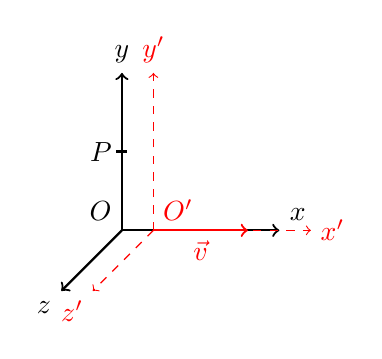
\begin{tikzpicture}[scale=2]
		\draw[thick,->] (0,0) node [above left]{$O$} -- (1,0) node[above right]{$x$};
		\draw[thick,->] (0,0) -- node [left,midway]{$P$} (0,1) node[above]{$y$};
		\draw[thick,->] (0,0,0) -- (0,0,1) node[below left]{$z$};
		\draw[thick] (-1pt,0.5) -- (1pt,0.5);
		
		\draw[red,dashed,->] (0.2,0) node [above right]{$O'$} -- (1.2,0) node[right]{$x'$};
		\draw[red,dashed,->] (0.2,0) -- (0.2,1) node[above]{$y'$};
		\draw[red,dashed,->] (0.2,0,0) -- (0.2,0,1) node[below left]{$z'$};
		
		\draw[thick,red,->] (0.2,0) -- (0.8,0) node [below,midway]{$\vec{v}$};
	\end{tikzpicture}
	\caption*{Changement de référentiels}
	\end{figure}
	\end{minipage}
	\begin{minipage}{0.45\textwidth}
		{\renewcommand*{\arraystretch}{1.2}$$
			\left\{ \begin{array}{r@{\;}l}
				ct'&=\gamma ct-\beta\gamma x\\
				x'&=-\beta\gamma ct+\gamma x\\
				y'&=y\\
				z'&=z
			\end{array} \right.
		$$}
	\end{minipage}
\end{center}

Les coordonnées de $P$ dans $\mathcal{R'}$ sont :
{\renewcommand*{\arraystretch}{1.2}$$
	\left\{ \begin{array}{r@{\;}l}
		ct'&=\gamma ct\\
		x'&=-\beta\gamma ct=-vt'\\
		y'&=b\\
		z'&=0
	\end{array} \right.
$$}
Dans $\mathcal{R'}$, le calcul du champ créé en $P$ est un problème d'électrostatique.
$$
	\left\{ \begin{array}{r@{\;}l}
		E'_x&=\frac{q}{4\pi\epsilon_0}\frac{x'}{r^3}\\
		E'_y&=\frac{q}{4\pi\epsilon_0}\frac{y'}{r^3}\\
		E'_z&=\frac{q}{4\pi\epsilon_0}\frac{z'}{r^3}
	\end{array} \right.	
	\kern 2cm B'_x=0=B'_y=B'_z\text{ avec }r'=\sqrt{x'^2+y'^2+z'^2}
$$
$$
	\text{Soit en P : }\left\{ \begin{array}{r@{\;}l}
		\vec{B}'&=\vec{0}\\
		E'_x&=\frac{q}{4\pi\epsilon_0}\frac{-vt'}{\sqrt{(-vt')^2+b^2}^3}\\
		E'_y&=\frac{q}{4\pi\epsilon_0}\frac{b}{\sqrt{(-vt')^2+b^2}^3}\\
		E'_z&=0
	\end{array} \right.
$$
et donc, pour le champ électromagnétique dans $\mathcal{R}$ au point $P$ :
$$
	\left\{ \begin{array}{r@{\;}l}
		E_x&=\frac{q}{4\pi\epsilon_0}\frac{-\gamma vt}{\sqrt{(\gamma vt)^2+b^2}^3}\\
		E_y&=\gamma E'_y=\frac{q}{4\pi\epsilon_0}\frac{\gamma b}{\sqrt{(\gamma vt)^2+b^2}^3}\kern 1cm \text{car }\vec{B}'=0\\
		E_z&=0
	\end{array} \right.	
$$
$$
	\begin{array}{r@{\;}l}
		B_x&=B'_x=0\\
		\vec{B_{\perp}}&=\gamma\left(\vec{B'_{\perp}}-\frac{\vec{ v}_{\mathcal{R}/\mathcal{R'}}\times\vec{E'_{\perp}}}{c^2}\right)\\
		&=-\gamma\frac{\vec{ v}_{\mathcal{R}/\mathcal{R'}}\times\vec{E'_{\perp}}}{c^2}\\
		&=-\frac{\vec{v}\times\vec{E}}{c^2}\\
		B_y&=0\\
		B_z&=\frac{1}{4\pi\epsilon_0 c^2}\frac{\gamma qvb}{\sqrt{b^2+(\gamma vt)^2}^3}
	\end{array}
$$
\end{app}
\begin{remarks}\hspace{1pt}
	\begin{itemize}
		\item comme $\vec{B'}=\vec{0}$, on a :
		$$
			\begin{array}{l@{\;}l}
				\vec{E_{\para}}&=\vec{E'_{\para}}\\
				\vec{E_{\perp}}&=\gamma\vec{E'_{\perp}} \kern 1cm \text{\emph{i.e.} la composante orthogonale est amplifiée d'un facteur }\gamma\\
				\vec{B}&=\frac{\vec{v}\times\vec{E}}{c^2}
			\end{array}
		$$
		\item Dans la limite où $\gamma \longrightarrow 1^+$, on retrouve la loi de Biot et Savart :
		$$
			\begin{array}{r@{\;}l}
				\vec{B}&=B_z\vec{u_z}\\
				B_z&=\frac{\mu_0}{4\pi}\frac{qvb}{\sqrt{b^2+(vt)^2}^3}\\
					&=\frac{\mu_0}{4\pi}\frac{q\vec{v}\times\vec{r}}{r^3}
			\end{array}\\
		$$
		\item {\txt On a $\frac{E_y}{E_z}=-\frac{b}{vt}$ qui est aussi la tangente de l'angle que fait $q\vec{P}$ avec $\vec{Ox}$, \emph{i.e.} les lignes de champ émanent de la position actuelle de la particule (et non la position retardée !)}
		\item On peut aussi écrire $\vec{E}$ après avoir introduit $\psi=(\vec{O'x'},\vec{O'P})$
		$$
			\vec{E}=\frac{q}{4\pi\epsilon_0}\frac{\vec{r}}{\gamma^2r^3(1-\beta^2\sin(\psi)^2)^{\frac{3}{2}}}
		$$
	\end{itemize}
\end{remarks}

\subsection{Invariants de Lorentz}
$F^{\mu\nu}$ est un tenseur gr\^ace auquel on peut construire tout sorte de tenseurs (par contraction, ou avec d'autres tenseurs). Parmi ceux-ci, deux présentent un intér\^et physique.
$$
	\begin{array}{l}
		\boxed{F_{\mu\nu}F^{\mu\nu}}\text{ : scalaire invariant}\\
		\boxed{\epsilon^{\mu\nu\rho\sigma}F_{\mu\nu}F_{\rho\sigma}}
	\end{array}		
$$
où $\epsilon^{\mu\nu\rho\sigma}$ est le tenseur totalement antisymétrique tel que :
$$
	\epsilon^{\mu\nu\rho\sigma}=\begin{cases}
		+1&\text{si }\mu\nu\rho\sigma\text{ est une permutation paire de }(0,1,2,3)\\
		-1&\text{si c'est une permutation impaire}\\
		0&\text{sinon}
	\end{cases}
$$
$$
	F_{\mu\nu}F^{\mu\nu}=\frac{2}{c^2}(c^2\vec{B}^2-\vec{E}^2)
$$

\begin{conc}
	$c^2\vec{B}^2-\vec{E}^2$ est un invariant.\\
	En particulier, si $c\|\vec{B}\|=\|\vec{E}\|$ dans un référentiel $\mathcal{R}$, alors $c\|\vec{B'}\|=\|\vec{E'}\| \kern 5pt \forall \kern 5pt \mathcal{R'}$ en translation rectiligne uniforme par rapport à $\mathcal{R}$. Cas particulier : pour une onde plane, on a $c\|\vec{B}\|=\|\vec{E}\|$, et donc, sans présumer du caractère plane dans $\mathcal{R'}$ on a : $c\|\vec{B'}\|=\|\vec{E'}\|$
\end{conc}
$$
	\begin{array}{r@{\;}l}
		\epsilon^{\mu\nu\rho\sigma}F_{\mu\nu}F_{\rho\sigma} &= 4!\text{ tenseurs}\\
			&=-\frac{8}{c}\vec{E}\cdot\vec{B}
	\end{array}
$$
\begin{conc}
	$\vec{E}\cdot\vec{B}$ est invariant
\end{conc}
\begin{app}
	Si dans $\mathcal{R}$ le problème est un problème d'électrostatique ($\vec{B}=\vec{0}, \kern 2pt c^2\vec{B}^2-\vec{E}^2<0$) ou de magnétostatique ($\vec{E}=\vec{0}, \kern 2pt c^2\vec{B}^2-\vec{E}^2>0$), alors $\forall \kern 2pt \mathcal{R'}$, on a $\vec{E}\cdot\vec{B}=0$. De m\^eme, pour une onde plane, $\vec{E}\cdot\vec{B}=0$, et donc dans $\mathcal{R'}$, et donc dans $\mathcal{R'}$, $\vec{E'}\cdot\vec{B'}=0$.
\end{app}
\begin{exo}
	Vérifier directement ces propriétés à partir des lois de transformation des champs.
\end{exo}

\section{Tenseur énergie-impulsion}
\subsection{Introduction}
On a été capable de donner une formulation covariante de la conservation de l'énergie-impulsion lorsque le système considéré est une charge :
$$
	\frac{dP^\mu}{d\tau}=qF^{\mu\nu}u_\nu
$$
Il est aussi possible d'écrire des lois de conservation pour l'énergie et pour l'impulsion lorsque le système considéré est la charge et un champ (\emph{cf.} notes). On essaie donc d'en donner une formulation covariante, d'abord en suivant une approche pédestre, puis en utilisant l'invariance du Lagrangien.

\subsection{Rappel des lois de conservation}
\begin{itemize}
	\item Conservation de l'énergie :
	$$
		\bigiiintsss \dif^3\vec{r}\left(\frac{\partial u}{\partial t}+\nab\cdot\vec{\Pi}+\vec{j}\cdot\vec{E}\right)=0
	$$
	$$
	\begin{array}{r@{\;}l}
		\text{avec }u(\vec{r},t)&=\frac{1}{2}\epsilon_0\vec{E}^2+\frac{1}{2\mu_0}\vec{B}^2\\
		\vec{\Pi}(\vec{r},t)&=\frac{\vec{E}\times\vec{B}}{\mu_0}
	\end{array}
	$$
	\item Conservation de l'impulsion
	$$
		\bigiiintsss \dif^3\vec{r}\left(\partial_j \mathcal{T}_{ij}-\partial_t\epsilon_0\left.(\vec{E}\times\vec{B})\right|_i\right)=\left.\frac{\partial\overrightarrow{P^v_{\text{part}}}}{\partial t}\right|_i
	$$
	$$
		\begin{array}{r@{\;}l}
			\mathcal{T}_{ij}&=\text{tenseur de Maxwell}\\
				&=\epsilon_0\left(E_iE_j+c^2B_iB_j-\frac{1}{2}(\vec{E}^2+c^2\vec{B}^2)\delta_{ij}\right)\\
				&\text{\hspace{2cm} avec }i,j\in\{x,y,z\}\\
			\overrightarrow{P^\nu_{\text{part}}} &= \text{impulsion locale des particules contenues dans }V\\
			\partial_t\overrightarrow{P^\nu_{\text{part}}}&=\iiint_V d^3\vec{r}\rho(\vec{E}+\vec{v}\times\vec{B})
		\end{array}
	$$
	$$
	\bigiiintsss \dif^3\vec{r}\left(\partial_j\mathcal{T}_{ij}-\partial_t\epsilon_0\left.(\vec{E}\times\vec{B})\right|_i\right) = \bigiiintsss \dif^3\vec{r}\rho\left.(\vec{E}+\vec{v}\times\vec{B})\right|_i
	$$
	Soit finalement :
	$$
	\boxed{
	\begin{array}{c}
		\frac{\partial u}{\partial t}+\nab\cdot\vec{\Pi} = -\vec{j}\cdot\vec{E}\\
		\partial_t\epsilon_0\left.(\vec{E}\times\vec{B})\right|_i+\partial_j(-\mathcal{T}_{ij})=-\rho\left	.(\vec{E}+\vec{v}\times\vec{B})\right|_i
	\end{array}}
	$$
\end{itemize}

\subsection{Tenseur énergie-impulsion du champ électromagnétique}
Calculons la quadri-force de Lorentz :
$$
	\boxed{f^\mu=F^{\mu\nu}J_\nu}
$$
$$
	\begin{array}{r@{\;}l}
		f^0&=F^{00}J_0+F^{01}J_1+F^{02}J_2+F^{03}J_3\\
			&=0+\left(-\frac{E_x}{c}\right)(-j_x)+\left(-\frac{E_y}{c}\right)(-j_y)+\left(-\frac{E_z}{c}\right)(-j_z)\\
			&=\frac{\vec{j}\cdot\vec{E}}{c}\\
		f^1&=F^{10}J_0+...\\
			&=\frac{E_x}{c}\rho c+0+(-B_z)(-j_y)+N_y(-j_z)\\
			&=\rho E_x +\rho v_yB_z-\rho v_zB_y\\
			&=\rho\left.(\vec{E}+\vec{v}\times\vec{B})\right|_x
	\end{array}
$$
Avec des résultats similaires pour $f^2$ et $f^3$. On s'attend par la forme des équations ($\partial t$ et $\nab$) et par analogie à la mécanique des flux (densité volumique de force $\leftrightarrow$ divergence du tenseur des contraintes) à voir apparaître à gauche un terme de la forme $\partial_\mu T^{\mu\nu}$

\begin{minipage}{0.45\linewidth}
$$
	\raggedleft
	\begin{array}{r@{\;}l}
		\frac{\partial u}{c\partial t}+\nab\cdot\frac{\vec{\Pi}}{c}&=-\frac{\vec{j}\cdot\vec{E}}{c}\\
			&=-f^0\\
			&=\partial_{\alpha}T^{0\alpha}
	\end{array}
$$
\end{minipage}\hspace{0.05\linewidth}
\begin{minipage}{0.40\linewidth}
$
	\text{avec }\left\{ \begin{array}{r@{\;}l}
		T^{00}&=\frac{1}{2}\epsilon_0\vec{E}^2+\frac{\vec{B}^2}{2\mu_0}\\
		T^{10}&=\frac{\Pi_x}{c}\\
		T^{20}&=\frac{\Pi_y}{c}\\
		T^{30}&=\frac{\Pi_z}{c}\\
	\end{array} \right.
$
\end{minipage}
\vspace{0.5cm}

\begin{minipage}{0.45\linewidth}
$$
	\begin{array}{r@{\;}l}
		\frac{\partial}{c\partial}\left(c\epsilon_0\left.(\vec{E}\times\vec{B})\right|_x\right)+\partial_j(-\mathcal{T}_{ij})&=-f^1\\
			&=\partial_{\alpha}T^{1\alpha}
	\end{array}
$$
\end{minipage}\hspace{0.05\linewidth}
\begin{minipage}{0.40\linewidth}
$
	\text{avec }\left\{ \begin{array}{r@{\;}l}
		T^{01}&=c\epsilon_0\left.(\vec{E}\times\vec{B})\right|_x=\frac{\Pi_x}{c}\\
		T^{11}&=-\mathcal{T}_{xx}\\
		T^{21}&=-\mathcal{T}_{xy}\\
		T^{31}&=-\mathcal{T}_{xz}\\
	\end{array} \right.
$
\end{minipage}

On trouve la même chose pour les composantes $y$ et $z$. Finalement, les quatre équations de conservation s'écrivent sous la forme :
$$
	\boxed{\partial_\mu T^{\mu\nu}=-F^{\nu\alpha}J_{\alpha}}
$$
où
$$
	T^{\mu\nu}=	\left( \begin{array}{cccc@{\/}}
		\frac{1}{2}\epsilon_0\vec{E}^2+\frac{\vec{B}^2}{2\mu_0} \kern 5pt & \kern 5pt \frac{\Pi_x}{c}  \kern 5pt & \kern 5pt  \frac{\Pi_y}{c}  \kern 5pt & \kern 5pt  \frac{\Pi_z}{c} \kern 5pt \\
		\begin{array}{c}
			\frac{\Pi_x}{c}\\
			\frac{\Pi_y}{c}\\
			\frac{\Pi_z}{c}
		\end{array} & \multicolumn{3}{c}{\left( \begin{array}{c}
			\\
			\kern 0.4cm \mathcal{T}_{\text{\tiny Maxwell}} \kern 0.4cm\\
			\\
		\end{array} \right)}
	\end{array} \right)
$$
avec
$$\mathcal{T}^{ij}_{\text{\tiny Maxwell}}=\epsilon_0\left(E_iE_j+c^2B_iB_j-\frac{1}{2}(\vec{E}^2+c^2\vec{B}^2)\delta_{ij}\right)$$

Il reste à vérifier que $T^{\mu\nu}$ est un tenseur.

\pagebreak

\begin{proof}\hspace*{1pt}
	\begin{itemize}
		\item \emph{Exercice.} Directement, en vérifiant que
		$$
			\tilde{T}^{\mu\nu}=\frac{\partial \tilde{x}^\mu}{\partial x^{\alpha}} \frac{\partial \tilde{x}^\nu}{\partial x^{\beta}} T^{\alpha\beta}
		$$
		\item En vérifiant que
		$$
			T^{\alpha\beta}=\frac{1}{\mu_0}\left(g^{\alpha\mu}F_{\mu\lambda}F^{\lambda\beta}+\frac{1}{4} g^{\alpha\beta}F_{\lambda\mu}F^{\lambda\mu}\right)
		$$
	\end{itemize}
\end{proof}

\begin{conc}
	$T^{\mu\nu}$ est effectivement un tenseur et la conservation de l'énergie-impulsion s'écrit sous forme covariante :
	$$
		\boxed{\partial_\mu T^{\mu\nu}=-F^{\nu\alpha}J_{\alpha}}
	$$
\end{conc}

\begin{remark}
	En relativité générale, on a :
	$$
		\begin{array}{l}
			R_{\mu\nu}-\frac{1}{2}g_{\mu\nu}R=8\pi gT_{\mu\nu}\\
			R_{\mu\nu} : \text{tenseur de Ricci}\\
			R^{\alpha}_{\mu\nu\alpha} : \text{tenseur de Riemann}\\
			R=R^{\alpha}_{\alpha}\text{, avec }R_{\alpha\beta\gamma\delta} :\text{fonction dérivée seconde de $g$ tenseur métrique}
		\end{array}
	$$

\end{remark}